% !TEX root =  paper.tex
\section{Experiments}

\begin{figure}[t]
	\centering
	\begin{minipage}{0.45\linewidth}
		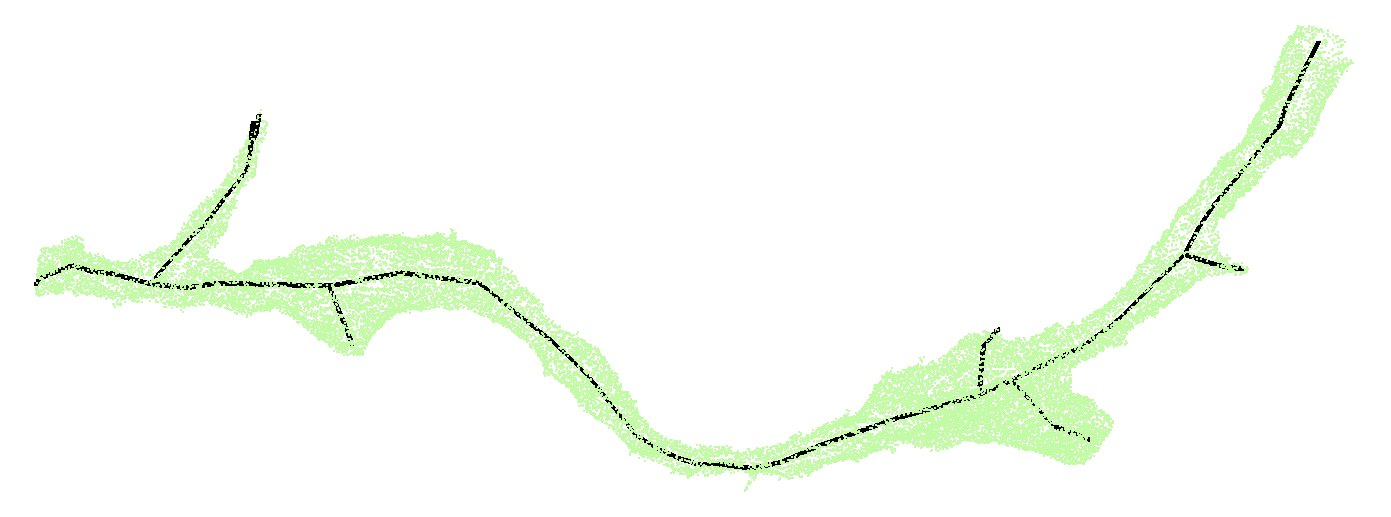
\includegraphics[width=\linewidth]{./figures/skeleton1.png}		
	\end{minipage}
	\hfill
	\begin{minipage}{0.45\linewidth}
		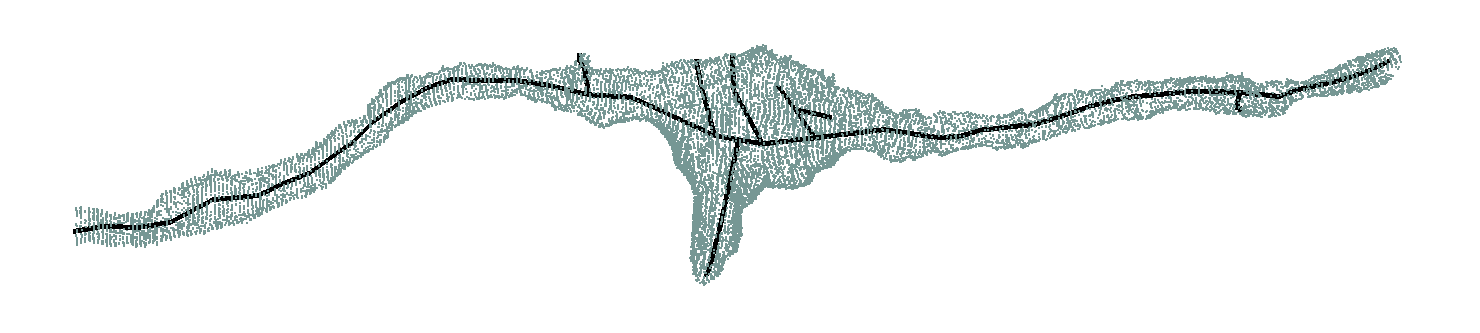
\includegraphics[width=\linewidth]{./figures/skeleton2.png}		
	\end{minipage}
	\begin{minipage}{0.45\linewidth}
		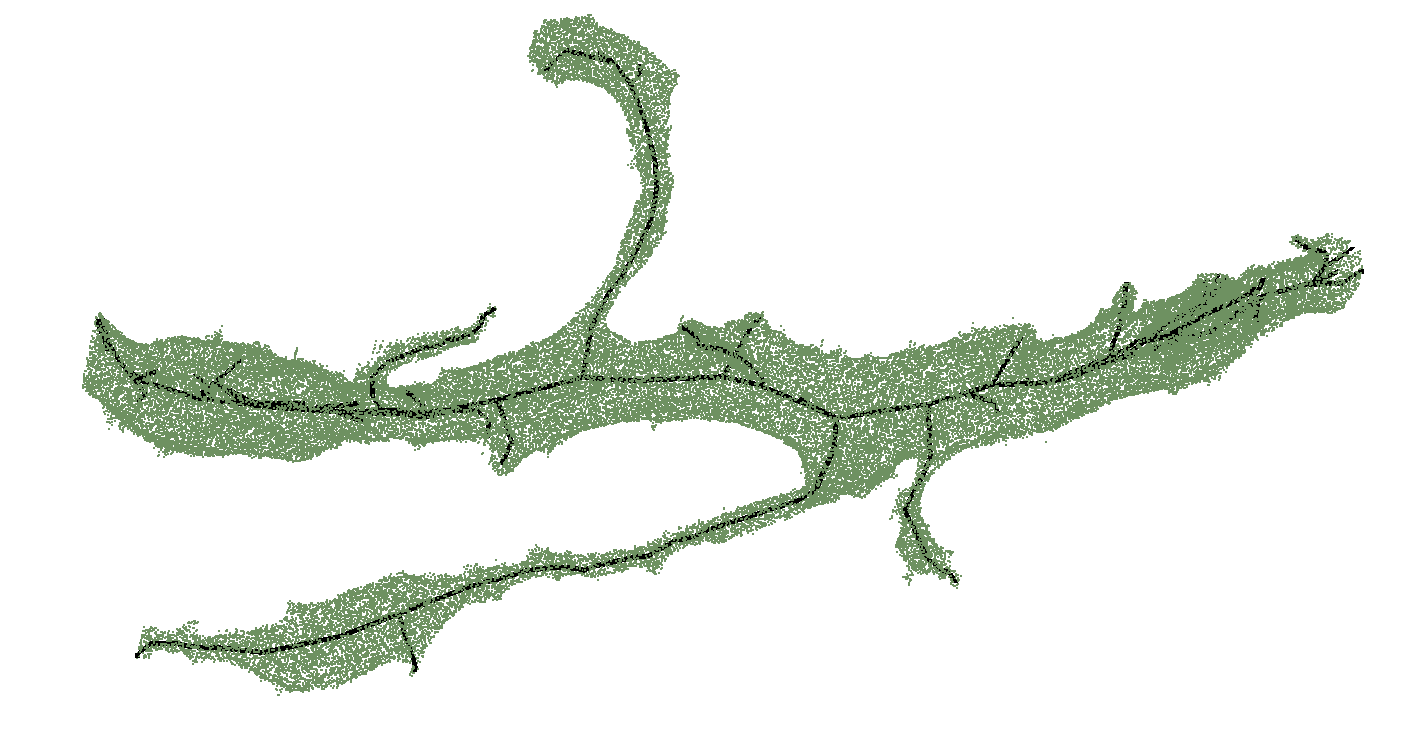
\includegraphics[width=\linewidth]{./figures/skeleton3.png}		
	\end{minipage}
	\hfill
	\begin{minipage}{0.45\linewidth}
		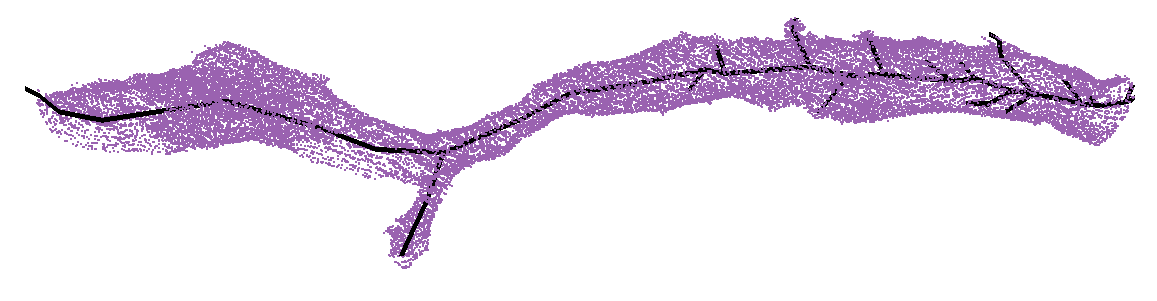
\includegraphics[width=\linewidth]{./figures/skeleton4.png}		
	\end{minipage}
	\caption{Example skeletons (in black) extracted from segments using a variant of the TEASER algorithm~\cite{sato2000teasar}. These skeletons not only capture the shape of the segmentation, but also provide endpoints useful for region merging proposals.}
	\label{fig:skeletonization}
\end{figure}

\begin{figure}[t]
	\begin{minipage}{0.4\linewidth}
		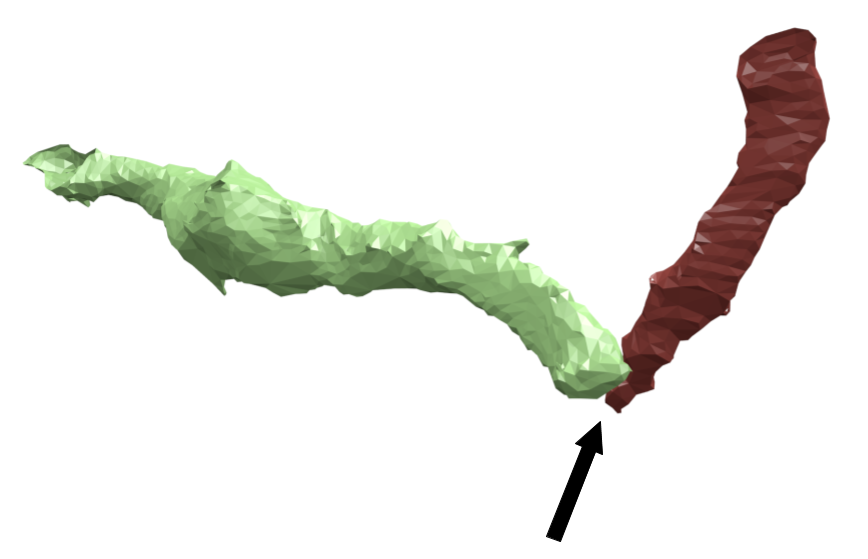
\includegraphics[width=\linewidth]{./figures/constraint_error.png}
	\end{minipage}
	\hfill
	\begin{minipage}{0.55\linewidth}
		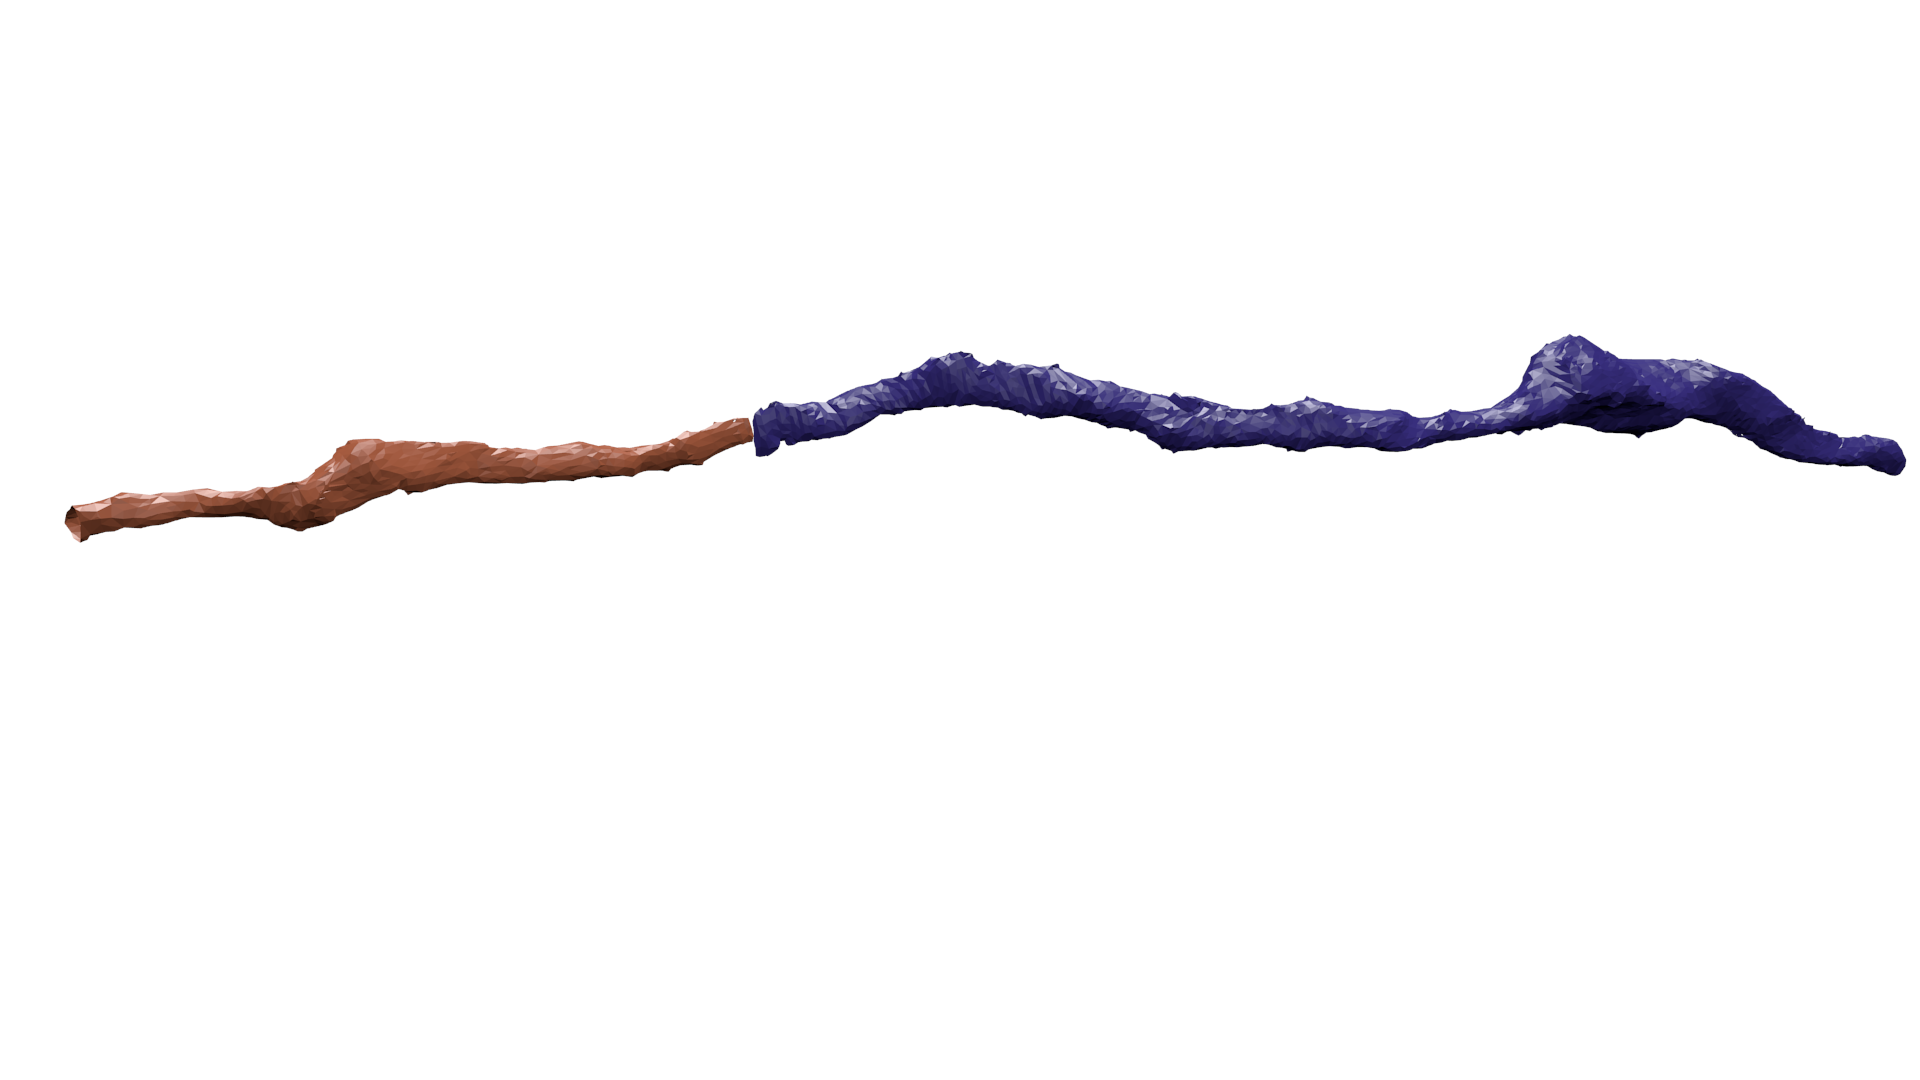
\includegraphics[width=\linewidth]{./figures/constraint_success.png}
	\end{minipage}
	\caption{Geometric constraints for region merging. We show two region merging proposals. On the left, the segments do not belong to the same neuron, as evidenced by the sharp turning radius indicated by the arrow; while on the right, the segments should be merged due to the continuity of the 3D shape. Instead of using handcrafted geometric features, we train a convolutional neural networks to automatically learn them from the ground truth labels.}
	\label{fig:turn-radii}
\end{figure}

\begin{figure}[t]
	\centering
	\begin{minipage}{0.32\linewidth}
		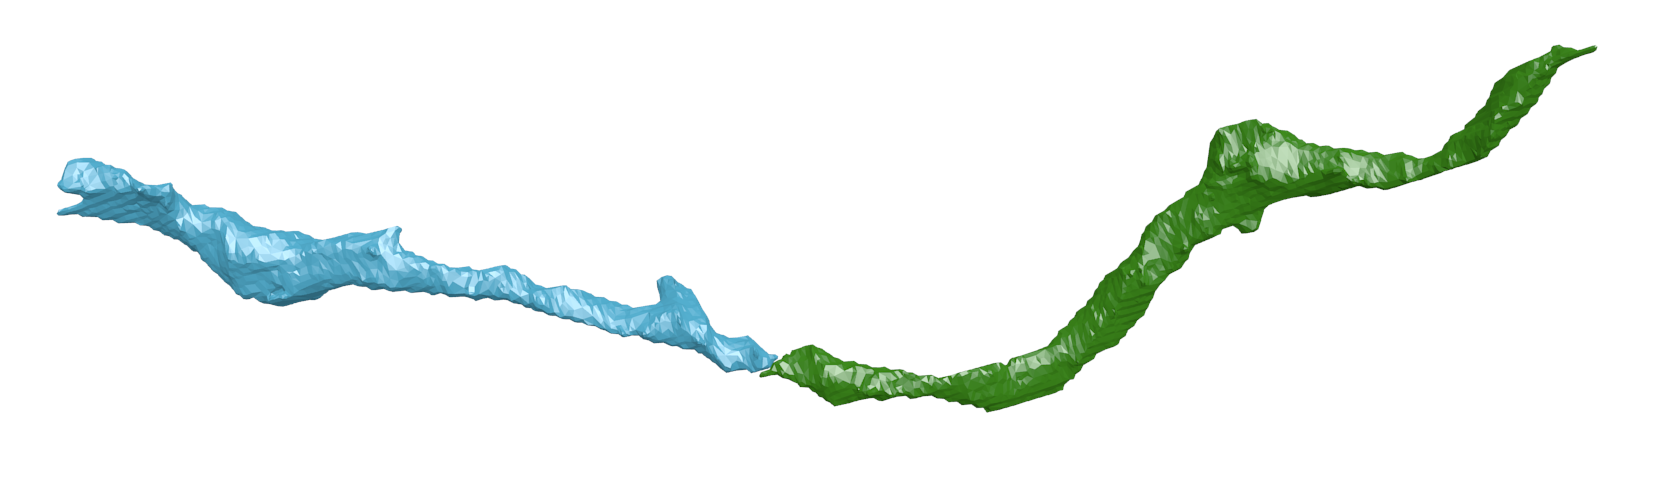
\includegraphics[width=\linewidth]{./figures/split_error1.png}		
	\end{minipage}
	\hfill
	\begin{minipage}{0.32\linewidth}
		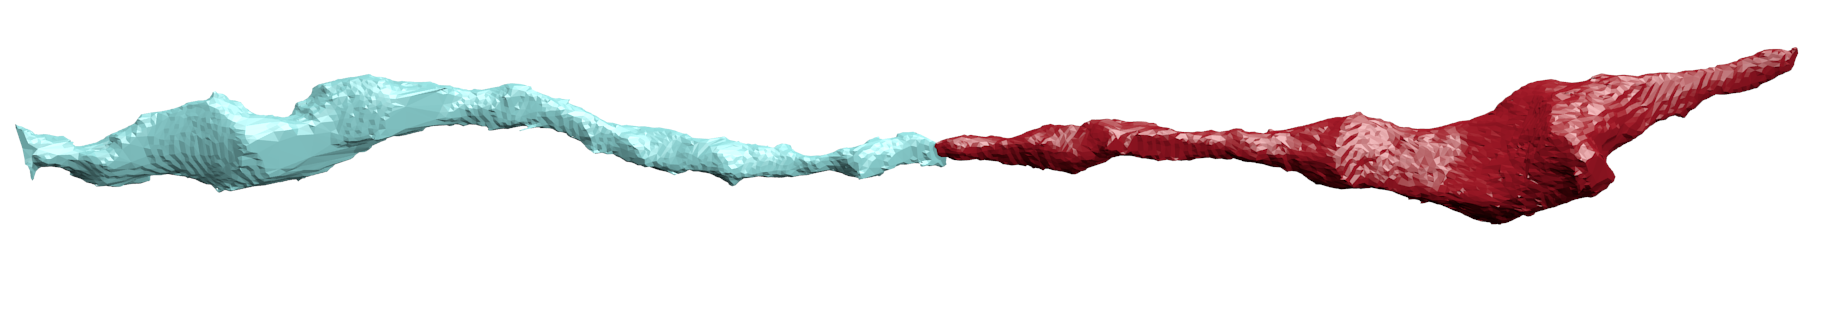
\includegraphics[width=\linewidth]{./figures/split_error2.png}				
	\end{minipage}
	\hfill
	\begin{minipage}{0.32\linewidth}
		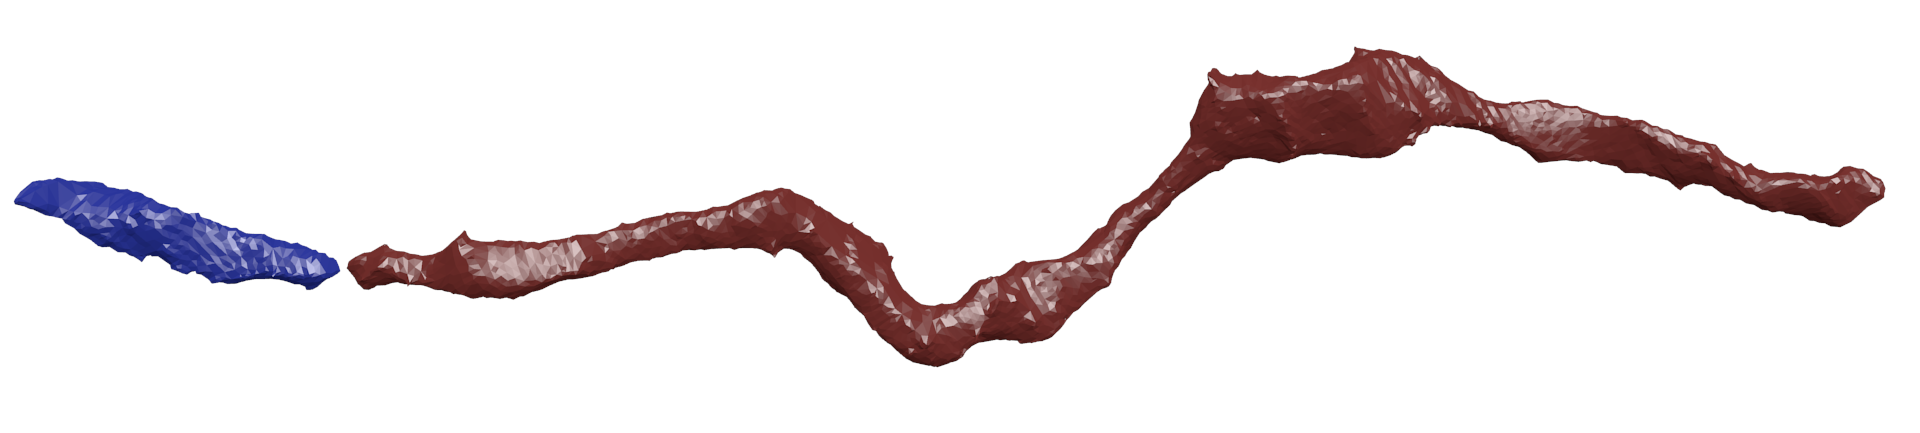
\includegraphics[width=\linewidth]{./figures/split_error3.png}
	\end{minipage}
	\caption{Three erroneously split segments.}
	\label{fig:merge_candidates}
\end{figure}


We evaluate our method by comparing it to a state-of-the-art pixel-based reconstruction approach using datasets from mouse and fly brains.

\subsection{Datasets}
\label{sec:dataset}

Our proposed method is designed for very large connectomics datasets. 
Popular challenge datasets such as CREMI and SNEMI3D are simply too small for any noticeable change. 
The following datasets contain 4 times more volume than the CREMI datasets. 
The first, which we call the Kasthuri dataset, consists of scanning electron microscope images of the neocortex of a mouse brain~\cite{kasthuri2015saturated}. 
This dataset is $5342 \times 3618 \times 338$ voxels in size. 
The resolution of the dataset is $\SI[product-units=single]{3 x 3 x 30}{\nano\meter}^3$ per voxel. 
We divide the dataset into two volumes (Vol. 1 and Vol. 2) along the $x$ dimension, where each volume is $\SI[product-units=single]{8.0 x 10.9 x 10.1}{\micro\meter}^3$.
We train one of these halves and test on the other.
Our second dataset, called FlyEM, comes from the mushroom body of a 5-day old adult male \textit{Drosophila} fly imaged by a focused ion-beam milling scanning electron microscopy~\cite{takemura2017connectome}.
The original dataset contains a $\SI[product-units=single]{40 x 50 x 120}{\micro\meter}^3$ volume with a resolution of $\SI[product-units=single]{10 x 10 x 10}{\nano\meter}^3$ per voxel. 
We use two cubes (Vol. 1 and Vol. 2) of size $\SI[product-units=single]{10 x 10 x 10}{\micro\meter}^3$.


\subsection{Method Configuration}
\noindent\textbf{Initial Segmentation}
The segmentation of the Kasthuri dataset is computed by agglomerating 3D supervoxels produced by the z-watershed algorithm from 3D affinity predictions~\cite{zlateski2015image}. 
A recent study by Funke et al.~\cite{funke2017deep} demonstrates superior performance of such methods over existing ones on anisotropic data. 
We learn 3D affinities using MALIS loss with a U-Net~\cite{ronneberger2015u,Turaga:2009}. 
We apply the z-watershed algorithm with suitable parameters to compute a 3D over-segmentation of the volume. 
The resulting 3D over-segmentation is then agglomerated using the technique of context-aware delayed agglomeration to generate the final segmentation~\cite{10.1371/journal.pone.0125825}.
For the FlyEM data, based on the authors' suggestion~\cite{takemura2017connectome}, we apply a context-aware delayed agglomeration algorithm~\cite{10.1371/journal.pone.0125825} that shows improved performance on this dataset over the pipeline used in the original publication. 
This segmentation framework learns voxel and supervoxel classifiers with an emphasis to minimize under-segmentation error. 
The algorithm first computes multi-channel 3-D predictions for membranes, cell interiors, and mitochondria, among other cell features. 
The membrane prediction channel is used to produce an over-segmented volume using 3D watershed, which is then agglomerated hierarchically up to a certain confidence threshold. 
We used exactly the same parameters as the publicly available code for this algorithm.
%For the Fib-25 challenge dataset, we use the segmentation from Funke et al. as our input~\cite{funke2017deep}.
\\~\\
\noindent\textbf{Graph Generation}
The two parameters for the graph pruning algorithm (Sec.~\ref{sec:skeletonization}) are $t_{low}$ and $t_{high}$. 
Ideally, our graph will have an edge for every over-segmented pair of labels with few edges between correctly segmented pairs. 
After considering various thresholds, we find that $t_{low} = \SI{210}{\nano\meter}$ and $t_{high} = \SI{300}{\nano\meter}$ produce expressive graphs with a scalable number of nodes and edges.
We explore these thresholds in greater detail in the supplemental material.
During implementation, we use nanometers instead of voxels for these thresholds to have uniform units across all datasets.
% Connectomics datasets often have lower sample resolutions in $z$ because of limitations during sample preparation. 
% Using nanometers allows us to have uniform units across all of these datasets and calculate the thresholds in voxels at runtime.
% Although the voxels vary between different datasets, the physical space remains constant. 
\\~\\
\noindent\textbf{Edge Weight Learning}
\label{sec:network-parameters}
We use half of the Kasthuri dataset for training and validation. 
We train on 80\% of the potential merge candidates for this volume.
We validate the CNN classifier on the remaining 20\% of the candidates. 
Since our input does not require the image data, we can train on the anisotropic Kasthuri data and test on the isotropic FlyEM data.

Since our input is an existing segmentation of the EM images, there are very few training examples compared to per-pixel classifiers that train on a unique window for each voxel. 
The Kasthuri dataset represents a region of brain over $\SI[product-units=single]{800}{\micro\meter}^3$ in volume and only yields 640 positive merge examples and 4821 negative ones.
To avoid overfitting our deep networks, we apply the following augmentations on the training examples.
During a single batch, we randomly select ten positive and ten negative examples. 
With probability 0.5, an example is reflected across the $xy$-plane. 
We then rotate each example by a random angle between $0$ and $360$ degrees using nearest neighbor interpolation. 
The supplemental material contains experiments demonstrating the benefits of this augmentation strategy.
We have 20,000 such examples per epoch.

\subsection{Error Metrics}
\label{sec:variation-of-information}
We evaluate the performance of the different methods using the split variation of information (VI)~\cite{meila2003comparing}.
Given a ground truth labeling $GT$ and our automatically reconstructed segmentation $SG$, over- and under-segmentation are quantified by the conditional entropies $H(GT | SG)$ and $H(SG | GT)$, respectively. 
Since we are measuring the entropy between two clusterings, lower VI scores are better.
The sum of these conditional entropies gives the total variation of information.

We use precision and recall to evaluate the convolutional neural network and multicut outputs. 
Since our method only corrects \textit{split errors}, we define a true positive as a pair of segments that are correctly merged together after our pipeline.